\chapter{Linear Collider Concepts}
\section{Luminosity}
Luminosity, $L$, is proportional to the number of collisions that are produced when two beams cross each other. The expression that relates luminosity, cross section $\sigma$ and the number of events produced $R$ is given by,
\begin{equation}
 R=L\sigma
\end{equation}
Luminosity will depend on the bunch population 	$N$ (assuming an equal number of particles for both beams) and their density distribution within the bunches 
% \section{Optics}
\section{Beam Delivery System (BDS)}
After the acceleration, in the Beam Delivery System (BDS) the beam needs to be focused and higher order aberrations must be compensated to obtain nanometer beam size. 
\section{Final Focus Sections (FFS)}
\section{Overview of FFS effects}
\subsection{Beamstrahlung}
\subsection{Hourglass effect}
Since the $\beta$-functions have their minimum at the IP and increase with the longitudinal distance, to consider the beam size constant along the whole collision length is some cases is not a good approximation. In a low-$\beta$ region 
\subsection{Crossing angle}
\subsection{Chromaticity}
As in the case of light beams through lenses, the longitudinal focal point location depends on the beam energy spread. This effect is called chromaticity.  Figure~\ref{f:chrom} represents schematically the focusing effect of a magnet as a lens. A particle with the design momentum crossing the lens at a distance $y_0$ from the center will be focused at $l^*$. Off-momentum particles with higher or lower momentum will be under-focused or over-focused, respectively. This produces a variation in the transverse position at the focal distance $l^*$ increasing the beam size.\par
\begin{figure}[!hbt]
\centering
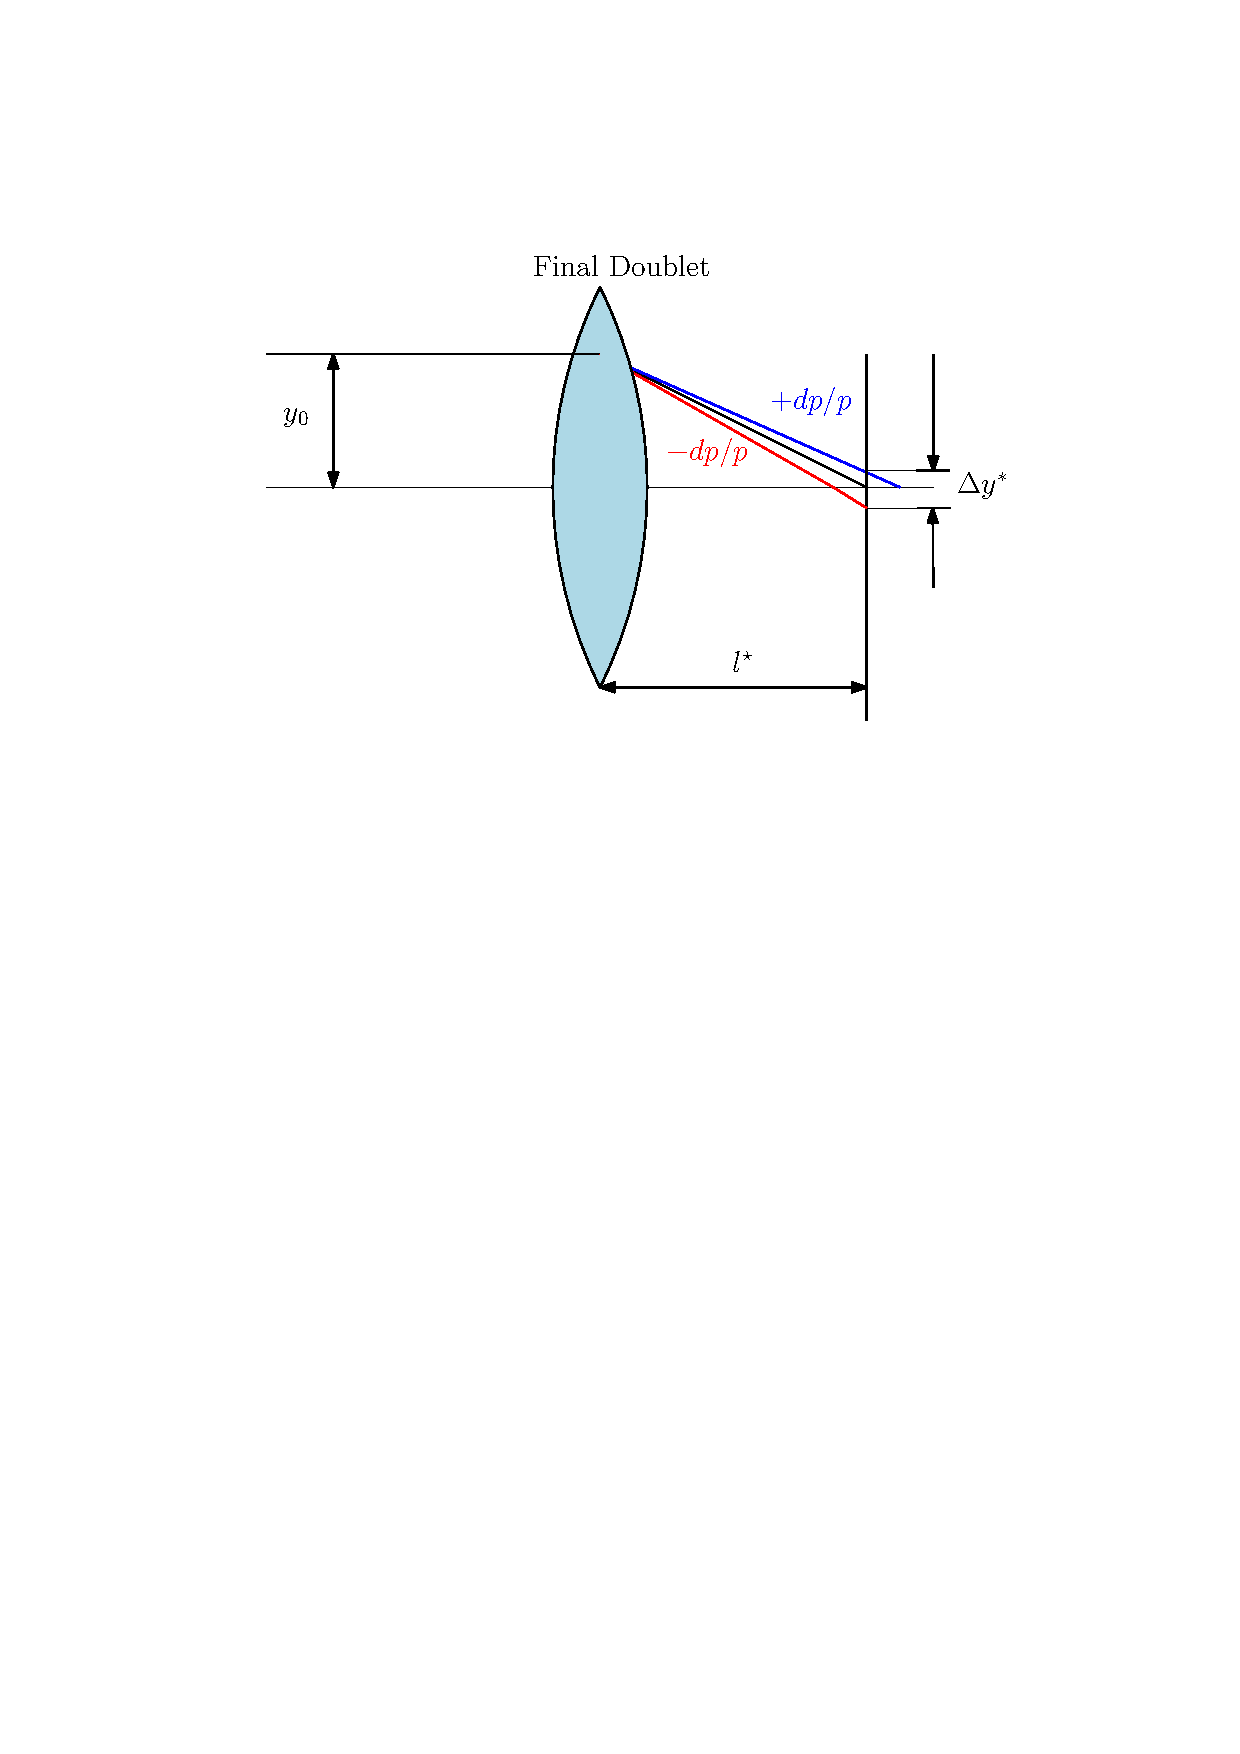
\includegraphics[scale=0.5]{chromaticity.pdf}\caption{Chromaticity. Particles with off-momentum energy are focused at different longitudinal locations increasing the beam size.}\label{f:chrom}
\end{figure}
The effect on the beam size is commonly estimated as
\begin{equation}
 \frac{\Delta y^*_{rms}}{\sigma^*_y}\approx\frac{l^*}{\beta^*}\sigma_\delta\approx\xi_y\sigma_\delta
\end{equation}
where $l^*$ is the focal length, $\sigma_\delta$ is the second moment of the energy spread distribution, $\beta_y^*$ is the optical $\beta$ function at the focal position and $\xi_y$ is the chromaticity.\par
The chromatic dilution of the beam size can be expressed as 
\begin{equation}
 \sigma^*_y\approx\sigma_{y,0}\sqrt{1+\xi_y^2\sigma^2_\delta}
\end{equation}
where $\sigma_{y,0}$ is the transverse beam size with zero energy spread.\par
\subsubsection{Chromaticity correction}\label{s:chromcorr}
In the thin lens approximation with a vertically focusing quadrupole magnet of thickness $ds$, the kick in angle given to a crossing particle is expressed in \cite{CAS9104} as
\begin{equation}
 dx'=k_q(1-\delta)xds\qquad dy'=-k_q(1-\delta)yds
\end{equation}
where $dx', dy'$ are the horizontal and vertical angle kick respectively, $k_q$ is the quadrupole gradient and $\delta=dP/P_0$ is the energy spread. A combination of bending magnets and sextupoles is used to substract the extra kick due to energy spread.\par
First, horizontal position and energy are correlated by dispersion, $\eta_x$, generated by bending magnets \cite{CAS9104}. This divides the particle motion in two parts: the betatron motion and an offset proportional to $\eta_x\delta$. Equation~(\ref{eq:coortrans}) shows the coordinate transformation.
\begin{align}
 x\rightarrow& x_\beta + \eta_x \delta\label{eq:coortrans}\\
 y\rightarrow& y_\beta\notag
\end{align}
Then, sextupoles are located in dispersive regions ($\eta_x\neq0$) to kick the particles cancelling the quadrupole angle kick dependence on energy. The quadrupole and sextupoles kicks in dispersive region are in Eq.~(\ref{eq:sextkick}), where $k_s$ is sextupole gradient.\par
\begin{align}
 \text{Quadrupole:}&\qquad dx'=k_q(1-\delta)(x_\beta+\eta_x\delta)ds\qquad& dy'=&-k_q(1-\delta)yds \label{eq:sextkick}\\
 \text{Sextupole:}&\qquad dx'=\frac{1}{2}k_s[(x_\beta+\eta_x\delta)^2+y_\beta^2]ds\qquad& dy'=&-k_s(x_\beta+\eta\delta)y_\beta ds\notag
\end{align}
The combination of bending magnets and sextupoles location and strengths are part of the lattice design. Two methods have been develop to achieve the cancellation of all second order terms in the transfer map: the non-local chromaticity correction and the local chromaticity correction.\par
\textbf{Non-local correction:}~The non-local correction scheme \cite{Brown:1988} compensates upstream the chromaticity in the Final Doublet (FD). Two pairs of sextupoles are used in horizontally dispersive regions ($\eta_x\neq0$) to compensate the particles path difference with respect to energy, explained in Section \ref{f:chrom}. They are matched to cancel geometrical components one to another by the -I transport map. Fig. (\ref{f-Non-local}) shows schematically the lattice configuration, where QF1 and QD0 constitute the FD, B0 to B5 are dipole magnets to produce horizontal dispersion, SD and SF sextupoles are used to cancel vertical and horizontal chromaticity respectively.\par
\begin{figure}[!htb]
   \centering
   \includegraphics*[scale=0.2,angle=0]{nonlocalcorr2.pdf}
   \caption{Non-local chromaticity correction.}
   \label{f-Non-local}
\end{figure}
\textbf{Local correction:}~The local chromaticity correction scheme \cite{Raimondi:2000} compensates chromaticity inside the FD and Fig. (\ref{f-local}) shows the sextupoles locations. Horizontal dispersion is generated in the FD to cancel second order dispersion and twice the chromaticity at the IP by matching the horizontal and vertical sextupoles gradients in the FD. For this reason,  chromaticity is created once more upstream in a non-dispersive region. An additional sextupole per plane is required to cancel only geometrical contributions to beamsize. As the vertical and horizontal corrections share the lattice section, this leads to a more compact design.\par
\begin{figure}[!htb]
   \centering
   \includegraphics[scale=0.2,angle=0]{localcorr2.pdf}
   \caption{Local chromaticity correction.}
   \label{f-local}
\end{figure}

\subsection{Tuning}
When considering imperfections, the machine performance decreases dramatically, typically, the beam size increases and luminosity drops substantially about 6 orders of magnitud. The tuning is the procedure which brings the system performance to its design values. Since the initial errors are unknown, the tuning requires a statistical study. Usually more than 100 machines with randomly distributed errors are considered in computer simulations. The simulated tuning reproduces a realistic tuning procedure in a machine \cite{GarciaMorales:1982827,Minty:629879}.\par
